\chapter{CƠ SỞ LÝ THUYẾT}

Chương cơ sở lý thuyết cung cấp những khái niệm nền tảng cho dự án, bao gồm khái niệm về Digital Twin, tổng quan về các giao thức M2M đang được dùng phổ biến hiện nay trong kết nối giữa máy và máy. Tiếp đến, thực nghiệm nhằm so sánh về hiệu năng dựa trên RTT giữa hai giao thức M2M phổ biến là MQTT và OPCUA được trình bày, cho ta thấy được sự khác biệt về hiệu năng giữa hai giao thức và nhấn mạnh được thế mạnh của giao thức OPCUA về khả năng đáp ứng được các điều kiện để trở thành một giao thức truyền thông mạnh mẽ, phù hợp trong môi trường công nghiệp. Sau cùng, nhóm trình bày những nghiên cứu liên quan với đề tài và nhắc lại kết quả cũng như hạn chế của đồ án chuyên ngành kĩ thuật máy tính trước đó, đây là những tài liệu tham khảo quý giá cho sự phát triển đồ án hiện tại của nhóm.

\section{Digital Twin}

%https://www.coursera.org/articles/digital-twin
%https://www.ibm.com/topics/what-is-a-digital-twin

% nếu đã phân loại các loại digital twin, thì em đánh giá digital twin của em là loại gì?

Công nghệ digital twin (Bản sao kĩ thuật số) là một khái niệm mới đang nổi lên, dần trở thành trung tâm của sự chú ý trong nền công nghiệp và dạo gần đây là trong các nghiên cứu. Sự phát triển của nền công nghiệp 4.0 và các công nghệ thời đại mới đã và đang tạo những bước phát triển lớn đối với nền công nghiệp thế giới. Internet of Things (IoT - mạng kết nối vạn vật) đã làm tăng lên số lượng dữ liệu được trao đổi trong hoạt động sản xuất, chăm sóc sức khỏe hay thành phố thông minh, từ đó tạo ra nhu cầu phân tích dữ liệu nhằm đưa ra những đánh giá, dự đoán, xác định lỗi, mô phỏng... Digital Twin xuất hiện như một giải pháp cho vấn đề tích hợp liền mạch giữa IoT và phân tích dữ liệu qua việc tạo ra sự kết nối giữa thực thể vật lý và bản sao ảo. Môi trường Digital Twin cho phép thực hiện các phân tích nhanh chóng và đưa ra quyết định thời gian thực thông qua những phân tích chính xác. Ở phần tiếp theo, ta sẽ tìm hiểu định nghĩa cụ thể của Digital Twin trong các giai đoạn lịch sử, và giải đáp những hiểu lầm thường thấy về Digital Twin. Tiếp đến, ta nhìn nhận những ứng dụng của Digital Twin trong thời đại công nghiệp 4.0, từ đó xác định những ưu, nhược điểm và thử thách của công nghệ này đối với sự phát triển của thời đại.


\subsection{Khái niệm về Digital Twin}

Khái niệm về Digital Twin đã xuất hiện từ khoảng những năm 2000. Cho đến nay, đã có những định nghĩa khác nhau về digital twin. Năm 2012, NASA \cite{glaessgen2012digital} cho rằng "Digital Twin là một mô phỏng tích hợp đa vật lý, đa cấp độ, mang tính xác suất (multiphysics, multiscale, probabilistic) của một phương tiện hay hệ thống đã tồn tại sử dụng mô hình tái hiện vật lý, cập nhật cảm biến, lịch sử... tốt nhất để ánh xạ sự tồn tại của vật thể đang bay". NASA đã từng hiện thực một digital twin cho tên lửa của họ trong chương trình Apollo, sau đó quân đội không quân Mĩ (US Air Force) cũng theo chân NASA và sử dụng công nghệ Digital Twin cho thiết kế, bảo trì và dự đoán sức khỏe các chiến cơ của họ. \cite{singh_origin_to_future}. Năm 2017, Chen \cite{chen2017integrated} cho rằng Digital twin là một mô hình vi tính hóa của một thiết bị vật lý hay hệ thống có khả năng thể hiện mọi chức năng và kết nối với các phẩn tử đang hoạt động". Zheng \cite{zheng2019application} định nghĩa Digital Twin như "Một tập thông tin ảo có khả năng mô tả tiềm năng hoặc quy trình sản xuất thực tế từ mức độ nguyên tử micro (micro atomic level) tới cấp độ hình học vĩ mô (macro geometrical level). Định nghĩa khác của của Madni \cite{madni2019leveraging} (2019) rằng "Digital Twin là một sự tồn tại ảo của một hệ thống vật lý luôn luôn được cập nhật với trạng thái, sự bảo trì và sức khỏe của hệ thống vật lý trong suốt vòng đời của nó." Theo nhóm, dù có nhiều định nghĩa khác nhau, nhưng chúng vẫn có chung các ý chính về Digital Twin là một bản sao ảo của vật thể ở thế giới thực, và bản sao này sẽ luôn luôn trao đổi, thu thập dữ liệu của vật thể thực nhằm phản ánh chân thực nhất trạng thái, sức khỏe của vật thể. Kèm theo đó, với dữ liệu thu thập được từ trạng thái của vật thế thật qua thực thể ảo, ta có thể sử dụng nó để đánh giá, phân tích, mô phỏng và đưa ra những quyết định phù hợp.

\subsection{Những nhầm lẫn về Digital Twin}

Digital Twin là một thực thể ảo trong môi trường ảo, phản ánh trạng thái của thiết bị thật và mang tính cá nhân hóa cao, nhưng điều đó không có nghĩa rằng chỉ cần tạo ra một mô hình ảo giống với thực tế thì là digital twin. Để làm rõ hơn về digital twin, Aidan Fuller \cite{fuller_dt_tech_challenge_research} đã phân tách những khái niệm thường bị nhầm lẫn khi nói về digital twin như sau:

\begin{figure}[!h]
    \centering
    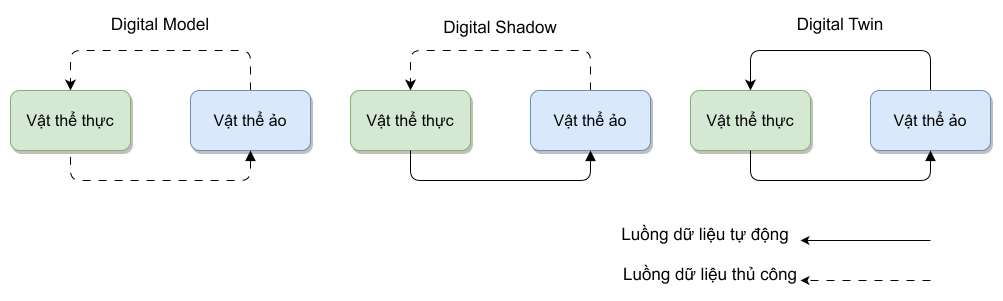
\includegraphics[width=1\textwidth]{Images/Methodologies/digital_twin_classification.png}
    \caption{Một số khái niệm nhầm lẫn của Digital Twin}
\end{figure}

\begin{itemize}
    \item \textbf{Mô hình ảo (Digital Model)}: Một mô hình ảo là một phiên bản số của một vật thể thực đã tồn tại hoặc dự định phát triển. Đối với một mô hình ảo, không hề có luồng dữ liệu tự động trao đổi giữa vật thể thực và mô hình ảo, một ví dụ thường thấy là mô hình ảo của tòa nhà, mô hình thiết kế hay phát triển sản phẩm. Điều này có nghĩa là thay đổi của vật thể thực sẽ không ảnh hưởng đến mô hình ảo, và ngược lại.
    \item \textbf{Bóng ma ảo (Digital Shadow)}: Bóng ma ảo bao gồm mô hình ảo của vật thế thực, nhưng lần này có thêm luồng dữ liệu từ vật thể thực sang mô hình ảo. Sự thay đổi trạng thái của vật thể thực sẽ ảnh hưởng tới mô hình ảo, nhưng không có chiều ngược lại.
    \item \textbf{Bản sao ảo (Digital Twin)}: Một mô hình ảo được gọi là digital twin khi có sự luân chuyển 2 chiều của dữ liệu, từ vật thể thực sang mô hình ảo và ngược lại. Điều này có nghĩa là thay đổi của vật thể thực cũng ảnh hưởng tới mô hình ảo, và thông qua mô hình ảo, ta có thể thay đổi, tác động lên vật thể thực.
\end{itemize}

\subsection{Ứng dụng của Digital Twin}

Digital Twin đã và đang được vận dụng trong nhiều lĩnh vực khác nhau. Khái niệm và định nghĩa của Digital Twin đang dần phát triển trong môi trường học thuật, cùng vói sự cải tiến không ngừng của các công nghệ IoT và AI. Hiện nay, ứng dụng được quan tâm chủ yếu của digital twin thường được thấy là các thành phố thông minh, sản xuất và một số ứng dụng liên quan tới sức khỏe \cite{fuller_dt_tech_challenge_research}

\subsubsection{Digital Twin trong thành phố thông minh}

Việc sử dụng và tiềm năng cho Digital Twin phát triển mạnh mẽ trong lĩnh vực thành phố thông minh đang tăng lên hằng năm nhờ vào sự phát triển nhanh của các kết nối thiết bị IoT. Với một lượng lớn các thành phố thông minh được xây dựng, sự kết nối giữa các cộng đồng càng cao, thì nhu cầu của digital twin cũng tăng cao. Lượng dữ liệu thu thập được từ các cảm biến IoT đang tích hợp trong các khu vực nhà thông minh cũng dần mở rộng, tạo đường cho những nghiên cứu nhắm tới xây dựng những thuật toán AI nâng cao.

Các dịch vụ và kiến trúc hạ tầng trong thành phố thông minh hoàn toàn có thể được cải thiện trong tương lai thông qua dữ liệu thu thập từ cảm biến được rải rác trong khu vực này. Dữ liệu có thể được sử dụng cho hỗ trợ việc thiết kế và phát triển các thành phố thông minh mới. Ngoài lợi ích đem lại trong việc thiết kế, dữ liệu còn giúp ích trong việc tiết kiệm năng lượng sử dụng. Chính sự phát triển của nhà thông minh, sự tăng lên của thiết bị IoT và dữ liệu thu thập đã và đang tạo ra tiềm năng ứng dụng công nghệ Digital Twin. Digital Twin giúp cải thiện tình trạng thành phố bằng cách tạo các mô phỏng sống trong môi trường ảo, thử nghiệm các kịch bản khác nhau, và đồng thời bản sao ảo của thành phố cũng học được từ môi trường thực tế bằng việc phân tích và giám sát dữ liệu nhận được.

\subsubsection{Digital Twin trong sản xuất}

Ứng dụng nổi bật tiếp theo của Digital Twin là trong môi trường sản xuất công nghiệp. Lý do chính cho việc này là do nhà sản xuất luôn cố gắng tìm cách kiểm soát và theo dõi việc sản xuất sản phẩm nhằm tìm giải pháp tiết kiệm thời gian và tiền bạc, là động lực và mục đích chính của mọi nhà sản xuất. Chính vì vậy, Digital Twin trở thành một lựa chọn hấp dẫn để ứng dụng trong môi trường sản xuất. Digital Twin mang lại khả năng cung cấp trạng thái thời gian thực về hiệu năng của máy móc và phản hồi của dây chuyền sản xuất, qua đó giúp cho nhà sản xuất tận dụng dữ liệu cho các dự doán, cải thiện và phát hiện vấn đề sớm hơn. 

Digital twin tăng cường kết nối và phản hồi giữa các thiết bị, qua đó, cải thiện độ tin cậy và hiệu năng. Digital Twin kết hợp với AI giúp tăng cường độ chính xác, khi digital twin không ngừng thu thập và lưu trữ lượng dữ liệu khổng lồ, từ đó được sử dụng bởi AI cho phân tích, dự đoán hiệu năng. Digital Twin cũng có thể tạo ra một môi trường để kiểm thử sản phẩm, hay một hệ thống hoạt động dựa trên dữ liệu thực tế thay vì dữ liệu giả định, giúp cho nhà sản xuất đưa ra những đánh giá, hành động hiệu quả và thực tế.

Một ứng dụng khác của digital twin được thực hiện hiện nay là trong ngành sản xuất ô tô, mà cụ thể bởi Tesla. Khả năng hiện thực một Digital Twin của bộ phận xe hơi trở nên rất giá trị vì có thể sử dụng bản sao ảo đó cho mô phỏng và phân tích dữ liệu. AI được sử dụng để phân tích dữ liệu thực tế trên xe, qua đó dự doán trạng thái hiện tại và tương lai của các bộ phận xe.

Ngành xây dựng cũng là một ngành thu được lợi ích từ việc ứng dụng Digital Twin. Theo dõi giai đoạn của công trình xây dựng hay thiết kế cấu trúc là những ứng dụng tiềm năng. Với việc theo dõi chất lượng công trình thật thông qua bản sao ảo, ta có thể biết được những thay đổi, ảnh hưởng của cấu trúc công trình, nhận biết sớm những vấn đề từ đó đưa ra bảo trì và sửa chữa nhanh chóng. Digital Twin cũng có thể được tạo ra trước khi xây dựng công trình, sử dụng những dữ liệu thực tế từ các công trình trước để thử nghiệm các mô phỏng

Điểm chung từ việc sử dụng digital twin trong các lĩnh vực trên là nhằm lợi dụng khả năng hiện thực mô phỏng thời gian thực sử dụng dữ liệu thực tế thay vì những model tĩnh thiếu chi tiết. Các model tĩnh cũng có tầm quan trọng của chúng, tuy nhiên thiếu sót các thông số thời gian thực và chi tiết sẽ làm giới hạn khả năng dự đoán và học hỏi. Digital Twin có thể học từ dữ liệu thực tế, dùng để quan sát trạng thái của vật thể thực, hay áp dụng lên nó những giải thuật học máy, học sâu.

\subsubsection{Digital twin trong chăm sóc sức khỏe}

Ngành chăm sóc sức khỏe là một lĩnh vực tiềm năng cho ứng dụng Digital Twin. Một ứng dụng tương lai có thể phát triển là Digital twin của cơ thể con người, đưa ra được dữ liệu thời gian thực của cơ thế. Ứng dụng thực tế hơn đang dùng hiện nay là sử dụng digital twin nhằm mô phỏng ảnh hưởng của một số loại thuốc, hay lập kế hoạch và thực hiện phẫu thuật.

Digital Twin trong chăm sóc sức khỏe đem lại khả năng giúp cho nhà nghiên cứu, bác sĩ, bệnh viện và dịch vụ chăm sóc sức khỏe mô phỏng môi trường cần thiết. Một lần nữa, Digital Twin có thể kết hợp với AI để đưa ra những dự đoán và quyết định chính xác. Sự phát triển của Digital Twin trong ngành này vẫn còn non yếu, tuy nhiên tiềm năng phát triển của nó vẫn rất cao, như việc quản lý giường bệnh tới quản lý bệnh viện.

Có thể thấy, Digital Twin vẫn là một ứng dụng tiềm năng cho thời đại công nghiệp 4.0, nhất là khi sự phát triển của IoT và AI đang có những bước tiến vượt bậc. Digital twin dự đoán sẽ đem lại nhiều đổi mới cho sản xuất và cách thức vận hành của doanh nghiệp. Ở phần đồ án này, nhóm sẽ tập trung nghiên cứu và ứng dụng một trong những khía cạnh quan trọng của Digital Twin, đó chính là giao thức hỗ trợ truyền tải dữ liệu sao cho đạt được khả năng truyền tải dữ liệu thời gian thực, nhanh và đáng tin cậy. Phần tiếp theo sẽ nói về các giao thức M2M (machine to machine) phổ biến đang được sư dụng hiện này trong môi trường công nghiệp, cụ thể là hai giao thức OPC UA và MQTT.

\section{Tổng quan về các giao thức M2M} 

Giao tiếp Machine-to-Machine (M2M) là một công nghệ đầy hứa hẹn cho các hệ thống giao tiếp thế hệ tiếp theo. Mô hình giao tiếp này tạo điều kiện cho các giao tiếp phổ biến với cơ chế tự động hóa hoàn toàn, trong đó một số lượng lớn thiết bị thông minh được kết nối bằng liên kết có dây/không dây, tương tác với nhau mà không cần sự can thiệp trực tiếp của con người. Do đó, giao tiếp M2M thường được ứng dụng trong các lĩnh vực rộng lớn như lưới điện thông minh, chăm sóc sức khỏe điện tử, mạng khu vực gia đình, hệ thống giao thông thông minh, giám sát môi trường, thành phố thông minh và tự động hóa công nghiệp. Để hiểu rõ hơn về công nghệ này, chúng ta sẽ cùng nhau tìm hiểu về Khái niệm, Cách thức hoạt động và Ứng dụng của nó trong đời sống.

\subsection{Giới thiệu về M2M}
M2M là viết tắt của “Machine to Machine.” Đó là một thuật ngữ mô tả bất kỳ công nghệ nào cho phép các thiết bị có kết nối mạng trao đổi thông tin và thực hiện các hành động mà không cần sự trợ giúp thủ công của con người. Nói cách khác, giao tiếp được thực hiện từ máy này sang máy khác.

Công nghệ M2M cho phép các thiết bị trên mạng đưa ra quyết định tự chủ mà không yêu cầu các thao tác thủ công. Mặc dù được sử dụng rộng rãi trong sản xuất, nhưng nó cũng được sử dụng trong các lĩnh vực khác. Các ứng dụng phổ biến bao gồm chăm sóc sức khỏe, bảo hiểm và Internet vạn vật (IoT).

Khi ở trong ngành sản xuất, nó thường được kết hợp với các công nghệ khác như SCADA. Một ví dụ về kết nối M2M trong các lĩnh vực khác là máy bán hàng tự động. Nó tự động gửi thông tin kiểm kê hàng trong kho của mình cho người điều phối. Một ví dụ điển hình khác là máy ATM tự gửi thông tin khi gần hết tiền mặt cho cơ quan chức năng của nó.

\subsection{Nguyên lý hoạt động của M2M}

Kết nối M2M có vẻ phức tạp, nhưng chúng hoạt động theo nguyên tắc đơn giản. Chúng lấy dữ liệu cảm biến tự động và chuyển dữ liệu đó qua mạng truy cập công cộng (public access network). Không giống như SCADA, các kết nối M2M sử dụng các mạng công cộng như mạng di động hoặc Ethernet. Đây là những gì làm cho các kết nối M2M trở nên hiệu quả về chi phí.

Một hệ thống M2M điển hình bao gồm nhiều cảm biến, RFID, Wi-Fi hoặc liên kết truyền thông di động (cellular communications link). Các cảm biến giao tiếp một số key condition với máy tính. Chẳng hạn, trong máy ATM, một cảm biến phát hiện mức tiền sẽ gửi tín hiệu khi tiền ở mức thấp.

Các hệ thống M2M cũng thường chứa phần mềm tính toán tự trị (autonomic computing software). Phần mềm này được thiết kế để giúp mạng diễn giải dữ liệu mà nó nhận được và hành động tương ứng.

Ngoài khả năng giám sát thiết bị và hệ thống từ xa, những lợi ích hàng đầu của M2M bao gồm:
\begin{itemize}
    \item \textbf{giảm chi phí} bằng cách giảm thiểu thời gian bảo trì và ngừng hoạt động của thiết bị;
    \item \textbf{tăng doanh thu} bằng cách mở ra các cơ hội kinh doanh mới để phục vụ các sản phẩm trong lĩnh vực này; và
    \item \textbf{cải thiện dịch vụ khách hàng} bằng cách chủ động theo dõi và bảo dưỡng thiết bị trước khi thiết bị hỏng hoặc khi cần thiết.
\end{itemize}

\subsection{Ứng dụng của M2M} 

% \begin{figure}[!h]
%     \centering
%     \includegraphics[width=0.8\textwidth]{Images/Basis_knowledge/m2m.jpg}
%     \caption{Ứng dụng của M2M \cite{m2mw}}
%     \label{fig:comp_mqtt}
% \end{figure} 

Kết nối M2M ở xung quanh chúng ta. Dưới đây là một vài ví dụ điển hình:

\textbf{Máy bán hàng tự động}
Một cảm biến phát hiện khi một sản phẩm cụ thể sắp hết trong máy bán hàng tự động. Thông tin này được truyền qua Wi-Fi hoặc mạng di động đến máy tính của người điều phối. Quá trình này hoàn toàn tự động.

\textbf{Y tế từ xa}
Trong lĩnh vực y tế từ xa, kết nối M2M có thể sử dụng các cảm biến để theo dõi thông tin quan trọng của bệnh nhân. Thông tin này sau đó có thể được chuyển đến một máy cục bộ gửi thuốc hoặc bác sĩ ở xa.

\textbf{Hệ thống nhà thông minh}
Có lẽ không lĩnh vực nào sử dụng kết nối M2M nhiều hơn hệ thống nhà thông minh. Có rất nhiều ví dụ về điều này. Điểm mấu chốt là nó cho phép một số cảm biến nhất định kết nối với các thiết bị khác để tự động hóa ngôi nhà của bạn.

\subsection{Giao thức MQTT}

\textbf{MQTT} (Message Queueing Telemetry Transport) được công bố là một giao thức cho các ứng dụng machine-to-machine theo mô hình publish/subscribe cực kì nhẹ và là một giao thức kết nối Internet of Things. Đây là một giao thức truyền thông điệp (message) mở, chủ yếu tập trung vào việc sử dụng băng thông thấp, độ tin cậy cao và có khả năng hoạt động trong điều kiện đường truyền không ổn định. Do đó, liên lạc giữa các cảm biến thông qua liên kết vệ tinh là một trong những ứng dụng của MQTT. Kể từ năm 2013, MQTT được tiêu chuẩn hóa thành một giao thức cho Internet of Things bởi Tổ chức Organization for the Advancement of Structured Information Standards (OASIS).

Mặc dù MQTT bắt đầu như một giao thức độc quyền được sử dụng để giao tiếp với các hệ thống thu thập dữ liệu và kiểm soát giám sát (SCADA) trong ngành dầu khí, nhưng nó đã trở nên phổ biến trong lĩnh vực thiết bị thông minh và ngày nay là giao thức nguồn mở hàng đầu để kết nối internet vạn vật ( IoT) và thiết bị IoT công nghiệp (IIoT).

\subsubsection{Nguyên lý hoạt động của MQTT}
Nhằm mục đích tối đa hóa băng thông có sẵn, mô hình giao tiếp publish/subscribe (pub/sub) của MQTT là một giải pháp thay thế cho kiến trúc client-server truyền thống - giao tiếp trực tiếp với điểm cuối. Ngược lại, trong mô hình pub/sub, ứng dụng khách gửi tin nhắn (message) (the publisher) được tách biệt khỏi các ứng dụng khách nhận tin nhắn (the subscribers). Bởi vì cả publisher và subscriber đều không liên hệ trực tiếp với nhau, nên bên thứ ba -- các broker -- sẽ chịu trách nhiệm cho các kết nối giữa chúng.

\begin{figure}[!h]
    \centering
    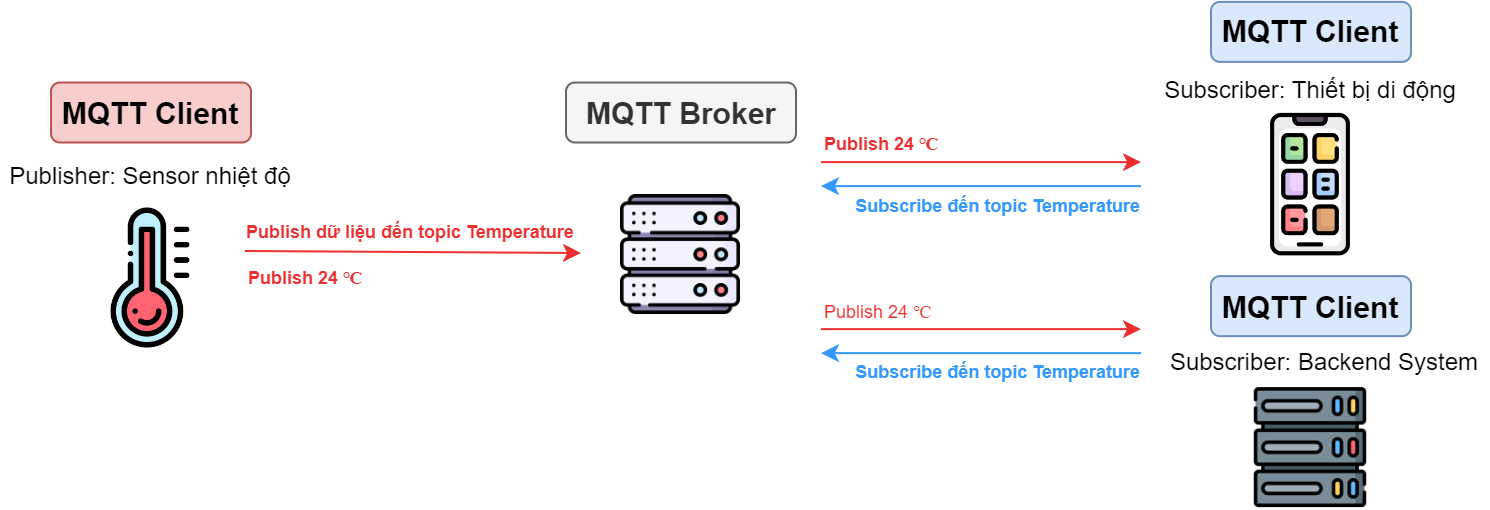
\includegraphics[width=\textwidth]{Images/Basis_knowledge/MQTTArchitec.png}
    \caption{Kiến thúc chung của MQTT sử dụng MQTT Broker}
    \label{fig:comp_mqtt}
\end{figure}

Ứng dụng khách MQTT (MQTT client) bao gồm publishers và subscribers, thuật ngữ này đề cập đến việc ứng dụng khách đang xuất bản tin nhắn (message) hay đăng ký nhận tin nhắn. Hai chức năng này có thể được triển khai trong cùng một máy khách MQTT. Khi một thiết bị (hoặc máy khách) muốn gửi dữ liệu đến máy chủ (hoặc broker), nó được gọi là \textit{publish}. Khi hoạt động được đảo ngược, nó được gọi là \textit{subscribe}. Theo mô hình pub/sub, nhiều client có thể kết nối với một broker và subscribe các \textit{topic} mà chúng quan tâm.

Một bài viết của IBM mô tả mô hình pub/sub: "Những Publisher gửi tin nhắn, những Subscriber nhận tin nhắn mà chúng quan tâm và Broker chuyển tin nhắn từ Publisher đến Subscriber. Publisher và Subscriber là ứng dụng khách MQTT (MQTT client), chỉ giao tiếp với một MQTT broker. Máy khách MQTT có thể là bất kỳ thiết bị hoặc ứng dụng nào (từ bộ vi điều khiển như Arduino đến máy chủ ứng dụng đầy đủ được lưu trữ trên Đám mây) chạy thư viện MQTT."\\

\textbf{Tin nhắn - Message}

Một cách khác để MQTT giảm thiểu quá trình truyền của nó là sử dụng cấu trúc message nhỏ, được xác định chặt chẽ. Mỗi message có một header cố định chỉ 2 byte. Có thể sử dụng header tùy chọn nhưng sẽ làm tăng kích thước của message. Tải trọng message được giới hạn chỉ 256 MB. Ba mức Chất lượng Dịch vụ (QoS) khác nhau cho phép các nhà thiết kế mạng lựa chọn giữa giảm thiểu truyền dữ liệu và tối đa hóa độ tin cậy.

\begin{figure}[!h]
    \centering
    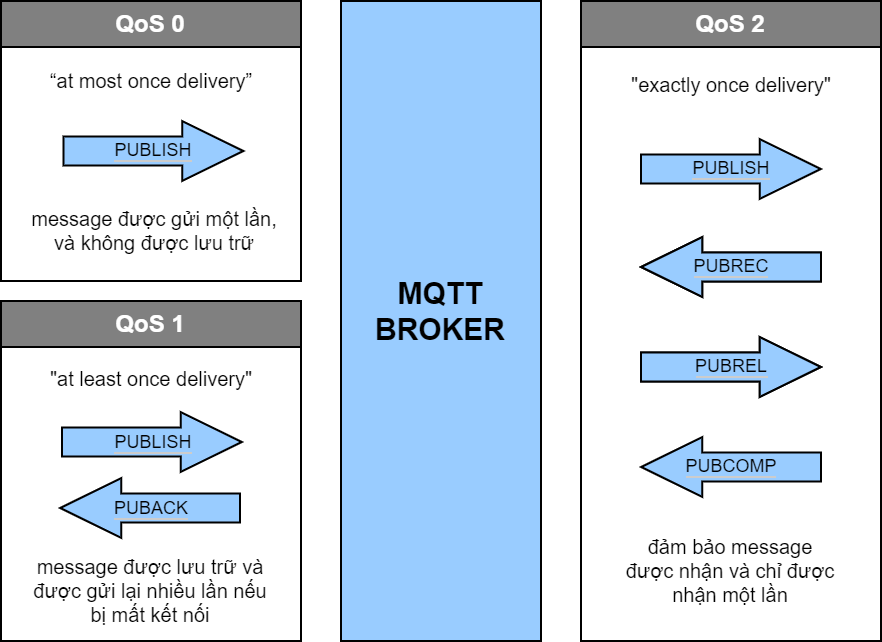
\includegraphics[width=0.8\textwidth]{Images/Basis_knowledge/QoS.png}
    \caption{Ba mức Chất lượng Dịch vụ (QoS)}
    \label{fig:comp_mqtt}
\end{figure}

\begin{itemize}
    \item \textbf{QoS 0} – Cung cấp lượng truyền dữ liệu tối thiểu. Với cấp độ này, mỗi message được gửi đến một subscriber một lần mà không cần xác nhận lại. Không có cách nào để biết liệu subscriber có nhận được tin nhắn hay không. Phương pháp này đôi khi được gọi là "fire and forget" hoặc "at most once delivery". Bởi vì cấp độ này giả định rằng quá trình gửi đã hoàn tất, nên các message không được lưu trữ để gửi cho các máy khách đã ngắt kết nối khi nó kết nối lại sau này.
    \item \textbf{QoS 1} – Broker gửi message và sau đó đợi phản hồi xác nhận từ subscriber. Nếu không nhận được xác nhận trong khung thời gian đã chỉ định, message sẽ được gửi lại. Sử dụng phương pháp này, subscriber có thể nhận được tin nhắn nhiều lần nếu broker không nhận được xác nhận của subscriber kịp thời. Và nó đôi khi được gọi là "at least once delivery".
    \item \textbf{QoS 2} – Client và broker sử dụng four-step handshake để đảm bảo rằng message được nhận và message đó chỉ được nhận một lần. Điều này được gọi là "exactly once delivery".
\end{itemize}

Đối với các trường hợp mà giao tiếp là đáng tin cậy nhưng tài nguyên bị hạn chế, thì QoS 0 có thể là lựa chọn tốt nhất. Đối với các trường hợp mà giao tiếp là không đáng tin cậy, nhưng khi các kết nối không bị giới hạn về tài nguyên, thì QoS 2 sẽ là lựa chọn tốt nhất. Còn QoS 1 là một loại giải pháp tốt cho cả hai trường hợp nhưng nó yêu cầu ứng dụng nhận dữ liệu phải biết cách xử lý các bản sao từ việc gửi message nhiều lần.

\textbf{Chủ đề - Topic}

\begin{figure}[!h]
    \centering
    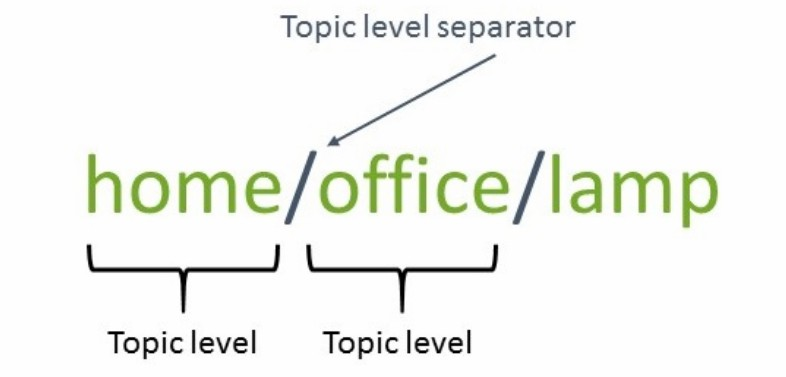
\includegraphics[width=0.5\textwidth]{Images/Basis_knowledge/topic.jpg}
    \caption{Cấu trúc của topic \cite{mqttw}}
    \label{fig:comp_mqtt}
\end{figure}
Message trong MQTT được publish dưới dạng topic. Các Topic là các cấu trúc trong hệ thống phân cấp sử dụng ký tự gạch chéo (/) làm dấu phân cách. Cấu trúc này tương tự như cấu trúc của cây thư mục trên hệ thống tệp máy tính. Một cấu trúc như \textbf{\textit{sensors/OilandGas/Pressure/}} cho phép subscriber chỉ định rằng chỉ nên gửi dữ liệu từ các máy khách publisher lên topic Pressure hoặc để có cái nhìn rộng hơn, có lẽ tất cả dữ liệu từ các máy khách publisher lên bất kỳ topic \textbf{\textit{sensors/OilandGas }} nào . Topic không được tạo rõ ràng trong MQTT. Nếu một broker nhận được dữ liệu được publish cho một topic hiện không tồn tại, topic đó sẽ được tạo đơn giản và client có thể subscribe topic mới.

\subsubsection{Ưu và Nhược điểm của MQTT}

\textbf{Ưu điểm}

Các thuộc tính lightweight và chi phí tối thiểu của kiến trúc giao thức MQTT giúp đảm bảo truyền dữ liệu trơn tru với băng thông thấp và giảm tải cho CPU và RAM. Các ưu điểm của MQTT so với các giao thức cạnh tranh như sau:
\begin{itemize}
    \item truyền dữ liệu hiệu quả và triển khai nhanh chóng do đây là một giao thức lightweight;
    \item mức sử dụng mạng thấp, do các gói dữ liệu được giảm thiểu;
    \item phân phối dữ liệu hiệu quả;
    \item thực hiện thành công remote sensing và điều khiển;
    \item truyền tải thông điệp nhanh chóng, hiệu quả;
    \item sử dụng lượng điện năng nhỏ, tốt cho các thiết bị được kết nối;
    \item tối ưu hóa băng thông mạng.
\end{itemize}

\textbf{Nhược điểm}

Nhược điểm tiềm ẩn đối với MQTT bao gồm:
\begin{itemize}
    \item MQTT có chu kỳ truyền chậm hơn so với Constrained Application Protocol (CoAP).
    \item Khám phá tài nguyên của MQTT hoạt động trên đăng ký chủ đề linh hoạt, trong khi CoAP sử dụng hệ thống khám phá tài nguyên ổn định.
    \item MQTT không được mã hóa. Thay vào đó, nó sử dụng TLS/SSL (Transport Layer Security/Secure Sockets Layer) để mã hóa bảo mật.
    \item Rất khó để tạo một mạng MQTT có thể mở rộng toàn cầu.
    \item Các thách thức khác liên quan đến bảo mật, khả năng tương tác và xác thực.
\end{itemize}

Do giao thức MQTT không được thiết kế với mục đích bảo mật nên giao thức này thường được sử dụng trong các mạng back-end an toàn cho các mục đích dành riêng cho ứng dụng. Cấu trúc topic của MQTT có thể dễ dàng tạo thành một cây khổng lồ và không có cách rõ ràng nào để chia cây thành các miền logic nhỏ hơn. Điều này gây khó khăn cho việc tạo ra mạng MQTT có thể mở rộng toàn cầu bởi vì khi kích thước của cây chủ đề tăng lên, độ phức tạp sẽ tăng lên.

Một nhược điểm khác của MQTT là thiếu khả năng tương tác (interoperability). Bởi vì payload của message là binary, nếu không có thông tin về cách chúng được mã hóa, thì các vấn đề có thể phát sinh -- đặc biệt là trong các kiến trúc mở, nơi các ứng dụng khác nhau từ các nhà sản xuất khác nhau hoạt động cùng nhau.

Như đã đề cập trước đây, MQTT có các tính năng xác thực tối thiểu được tích hợp trong giao thức. Tên người dùng và mật khẩu được gửi ở dạng văn bản rõ ràng và bất kỳ hình thức sử dụng MQTT an toàn nào cũng phải sử dụng SSL/TLS, và thật không may, đây không phải là một giao thức nhẹ.

Xác thực ứng dụng khách (client) bằng client-side certificate không phải là một quy trình đơn giản và MQTT không có cách nào để kiểm soát ai sở hữu topic và ai có thể publish thông tin trên đó, ngoại trừ sử dụng các phương tiện độc quyền (proprietary), ngoài băng tần (out-of-band). Điều này giúp dễ dàng đưa các message có hại vào mạng, do cố ý hoặc do nhầm lẫn.

Hơn nữa, không có cách nào để người nhận message biết ai đã gửi message gốc trừ khi thông tin đó có trong message. Các tính năng bảo mật phải được triển khai trên MQTT theo kiểu độc quyền sẽ làm tăng code footprint và khiến việc triển khai trở nên khó khăn hơn.

\subsubsection{Ứng dụng của MQTT}
Do các đặc tính nhẹ của nó, MQTT hoạt động tốt cho các ứng dụng liên quan đến giám sát từ xa, bao gồm:
\begin{itemize}
    \item đồng bộ hóa các cảm biến, chẳng hạn như đầu báo cháy hoặc cảm biến chuyển động để phát hiện hành vi trộm cắp, để xác định xem mối nguy hiểm có hợp lệ hay không;
   \item theo dõi các thông số sức khỏe bằng cảm biến cho các bệnh nhân đã xuất viện;
   \item cảm biến cảnh báo con người về sự nguy hiểm.
\end{itemize}

% \begin{figure}[!h]
%     \centering
%     \includegraphics[width=0.9\textwidth]{Images/Basis_knowledge/MQTTapplication.jpg}
%     \caption{Ứng dụng của MQTT \cite{mqtttechw}}
%     \label{fig:comp_mqtt}
% \end{figure}

Một ứng dụng khác là ứng dụng nhắn tin dựa trên văn bản để liên lạc theo thời gian thực, tận dụng mức sử dụng năng lượng và dữ liệu thấp của MQTT. Ví dụ: Facebook sử dụng MQTT cho ứng dụng Messenger của mình, không chỉ vì giao thức này tiết kiệm pin trong khi nhắn tin từ điện thoại đến điện thoại mà còn vì giao thức này cho phép gửi tin nhắn hiệu quả trong một phần nghìn giây, mặc dù kết nối internet không nhất quán trên toàn cầu.

Hầu hết các nhà cung cấp dịch vụ đám mây, bao gồm Amazon Web Services (AWS), Google Cloud, IBM Cloud và Microsoft Azure, đều hỗ trợ MQTT.

MQTT rất phù hợp với các ứng dụng sử dụng thiết bị M2M và IoT cho các mục đích như phân tích thời gian thực, bảo trì và giám sát phòng ngừa trong các môi trường, bao gồm nhà thông minh, chăm sóc sức khỏe, logistics, công nghiệp và sản xuất.

\subsection{Giao thức OPC-UA}

\textbf{OPC UA} (Open Platform Communications Unified Architecture) là một giao thức truyền thông machine-to-machine theo hướng dịch vụ, chủ yếu được sử dụng trong tự động hóa công nghiệp và được định nghĩa trong IEC 62541. Các mục tiêu chính của nó là cung cấp một giao thức truyền thông đa nền tảng khi sử dụng mô hình thông tin để mô tả dữ liệu được truyền. Các tính năng và thành phần khác nhau của OPC UA được mô tả trong các phần đặc tả kỹ thuật khác nhau do OPC Foundation phát hành và công bố rộng rãi . OPC UA chủ yếu được thúc đẩy bởi ngành công nghiệp sản xuất ở Châu Âu, do đó nó ngày càng giành được vị trí quan trọng lĩnh vực này, đồng thời nó cũng đang trở thành một trong những giao thức trọng yếu trên toàn thế giới. Điểm mạnh chính của OPC UA là mô tả ngữ nghĩa của mô hình không gian địa chỉ cùng với những thông số kỹ thuật đồng hành khác nhau giúp mở rộng các mô tả ngữ nghĩa cơ bản cho các miền khác nhau như PLCopen, robot hoặc thị giác máy tính.
   
\subsubsection{Nguyên lý hoạt động của OPC UA}

OPC UA cho phép việc truy cập đến các máy tính, thiết bị và các hệ thống khác, tổ chức dữ liệu theo hướng có cấu trúc, chi tiết và được xây dựng theo kiến trúc hướng dịch vụ giúp OPC-UA là một lựa chọn chủ yếu trong môi trường công nghiệp. Ở phần này ta sẽ tìm hiểu sâu về các thành phần của OPC UA và cách hoạt động của nó.\\

\textbf{Model}

Sử dụng các mô hình, OPC UA chỉ định các quy tắc cơ bản để hiển thị dữ liệu cho bất kỳ ứng dụng hoặc thiết bị nào muốn sử dụng nó. Bản thân OPC UA là một mô hình dữ liệu tập trung vào thông tin (information-centric data). Nó bao gồm một mô hình đối tượng chung (generic object model) với một hệ thống kiểu có thể mở rộng với các mô hình tích hợp để truy cập dữ liệu. Các mô hình tích hợp này chỉ định các chức năng như thông tin báo động và sự kiện, thông tin về dữ liệu lịch sử, chi tiết truy cập dữ liệu, mô tả thiết bị và để thực thi các chương trình.

Dữ liệu cũng có thể được truy cập thông qua các mô hình tùy chỉnh, được gọi là mô hình đồng hành (companion model). Chúng được sử dụng trong các ngành công nghiệp khác nhau như sản xuất máy ép phun hoặc kỹ thuật chế tạo robot.\\

\textbf{Luồng dữ liệu và kết nối}

OPC UA hỗ trợ giao tiếp giữa các thành phần ở năm level (Hình 2.7) trong các tổ chức công nghiệp: enterprise, management, operations, control, and field (thiết bị dành riêng cho nhà cung cấp).

\begin{figure}[!h]
    \centering
    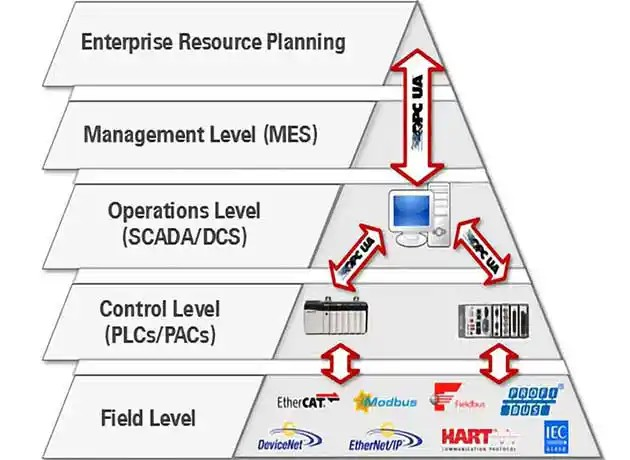
\includegraphics[width=0.7\textwidth]{Images/Basis_knowledge/industrial_levels.jpg}
    \caption{Năm level trong tổ chức công nghiệp \cite{5levw}}
    \label{fig:comp_mqtt}
\end{figure}

Các thiết bị hiển thị dữ liệu của chúng thông qua OPC UA, cho phép vận chuyển thông tin này qua mạng tới một ứng dụng tiêu thụ bằng các dịch vụ web tiêu chuẩn. Dữ liệu được vận chuyển bằng các giao thức dựa trên IP và SOAP nhờ đó các máy chủ cấp thấp (low-end server) có thể sử dụng UA TCP. Việc sử dụng các dịch vụ web SOAP tiêu chuẩn qua HTTP cho phép các máy khách không thuộc OPC UA có thể yêu cầu dữ liệu do máy chủ OPC UA publish.

Phần mềm cầu nối và cổng (Bridging and gateway software) được gọi là OPC UA wrappers cho phép luồng dữ liệu trên phần cứng dành riêng cho nhà cung cấp giữa các OPC UA level. OPC UA wrappers cũng có thể được sử dụng để chuyển đổi từ OPC Classic sang OPC UA hoặc khi máy chủ OPC hỗ trợ UA nhưng máy khách OPC thì không.\\

\textbf{Kiến trúc hướng dịch vụ (Service-oriented architecture) - SOA}

OPC UA giao tiếp dựa trên SOA client-server framework. Trong OPC UA, có máy chủ OPC UA (OPC UA servers) và máy khách OPC UA (OPC UA clients).

\textbf{Máy chủ OPC UA (OPC UA server)} là cơ sở của giao tiếp OPC UA. Nó là một phần mềm triển khai tiêu chuẩn OPC và từ đó cung cấp các giao diện OPC được tiêu chuẩn hóa cho thế giới bên ngoài. Máy chủ OPC UA cung cấp cho máy khách OPC UA các ứng dụng và hệ thống điều khiển, ví dụ như MES và SCADA, đồng thời có quyền truy cập an toàn vào dữ liệu tự động hóa công nghiệp bằng cách sử dụng các mô hình thông tin OPC UA chỉ định cách tổ chức, lưu trữ và thu thập dữ liệu. Thuật ngữ máy chủ OPC UA đề cập đến \textbf{tiêu chuẩn phần mềm OPC UA trên máy} chứ không phải bản thân phần cứng, có thể là một máy chủ ảo.

\begin{figure}[!h]
    \centering    
    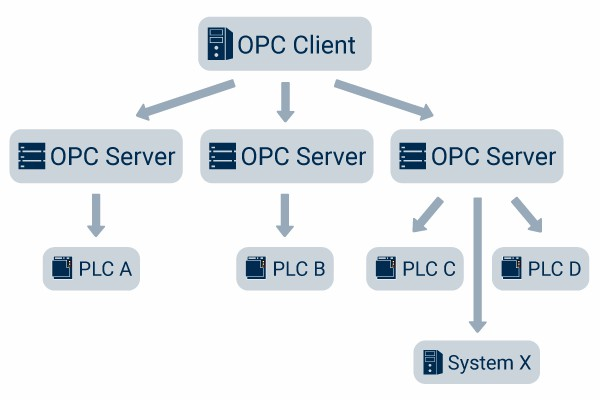
\includegraphics[width=0.8\textwidth]{Images/Basis_knowledge/OPC_server.jpg}
    \caption{OPC UA server \cite{opcrw}}
    \label{fig:comp_mqtt}
\end{figure}

\textbf{Máy khách OPC UA (OPC UA client)} là máy khách có thể hỗ trợ mô hình thông tin OPC UA. Máy khách OPC UA yêu cầu dữ liệu và ghi dữ liệu vào các thành phần trong hệ thống thông qua máy chủ OPC UA. Do các Máy chủ OPC UA triển khai các giao diện được xác định trước của tiêu chuẩn OPC UA nên mỗi máy khách có thể truy cập bất kỳ Máy chủ OPC UA nào và trao đổi dữ liệu với máy chủ theo cùng một cách.

\begin{figure}[!h]
    \centering
    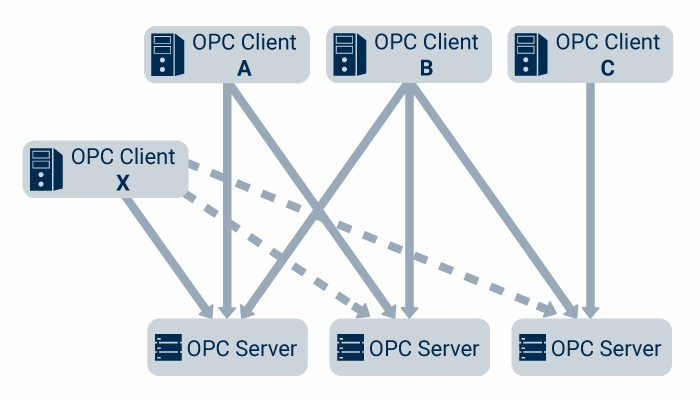
\includegraphics[width=0.8\textwidth]{Images/Basis_knowledge/OPC_client.jpg}
    \caption{OPC UA client \cite{opcrw}}
    \label{fig:comp_mqtt}
\end{figure}

Các hệ thống SOA như OPC UA tích hợp các ứng dụng khác nhau qua mạng và kết nối các thiết bị trên các nút mạng khác nhau.\\

\newpage
\textbf{Node}

Node là đơn vị dữ liệu cơ bản trong không gian địa chỉ OPC UA, cung cấp một cách tiêu chuẩn cho các máy chủ OPC UA để biểu diễn các đối tượng cho các máy khách OPC UA. Các Node là các mẩu thông tin (ví dụ: nhiệt độ) và bao gồm các thuộc tính, giá trị dữ liệu thực và một hoặc nhiều tham chiếu đến các Node khác, mỗi Node nằm trong không gian địa chỉ riêng của nó. Do đó, một mẩu thông tin về nhiệt độ sẽ chiếm nhiều địa chỉ trong một không gian địa chỉ.

Các Node được tham chiếu bởi một Node ID duy nhất: một namespace URI (số nhận dạng tài nguyên duy nhất), loại dữ liệu (data type) và số nhận dạng (identifier). Mỗi Node thuộc về một namespace cụ thể. Namespace URI được đặt trong một bảng namespace riêng trên máy chủ OPC UA. Bảng namespace lưu trữ các URI riêng biệt cho các mô hình thông tin được sử dụng bởi các tổ chức riêng lẻ có yêu cầu riêng về việc dữ liệu sẽ trông như thế nào và hoạt động ra làm sao. Điều này cho phép OPC UA mở rộng các dịch vụ của mình mà không thay đổi thiết kế cơ bản của tiêu chuẩn.

Trong OPC UA, các Node có nhiều lớp cho phép tạo các biến thể trên Node cơ bản. Các lớp Node đối tượng trong OPC UA là chìa khóa để nó có thể tạo dữ liệu phức tạp và phân biệt giữa các thực thể tương tự nhưng khác nhau, ví dụ như cảm biến nhiệt độ cho máy điều hòa không khí và cảm biến nhiệt độ cho nồi hơi.

\subsubsection{Ưu và nhược điểm của OPC UA}

\textbf{Ưu điểm}

\begin{itemize}
    \item \textbf{Phân quyền}\\
    Về mặt lịch sử, kim tự tháp tự động hóa trong các hệ thống công nghiệp là một cấu trúc phân cấp mô tả luồng thông tin từ các thiết bị cấp thấp như bộ điều khiển, cảm biến hoặc đồng hồ đo đến các ứng dụng ERP cấp cao. Ở hướng ngược lại là một luồng kiểm soát, từ các ứng dụng ERP cấp cao đến các thiết bị cấp thấp. Các thành phần cấp thấp được kết nối qua mạng MES thông qua PLC và HMI.\\
    OPC UA loại bỏ cấu trúc kim tự tháp này bằng cách phi tập trung hóa các thành phần hệ thống và tạo điều kiện thuận lợi cho việc sử dụng các cấu trúc mô hình hóa dữ liệu linh hoạt hơn trong mạng lưới. OPC UA đạt được điều này bằng cách xác định cấu trúc dữ liệu nhất quán mà tất cả các thành phần sử dụng, ví dụ: ứng dụng ERP và cảm biến trường đều có thể sử dụng cùng một mô hình thông tin.
    \item \textbf{Nền tảng độc lập}\\
    Trước đây, các hệ thống công nghiệp chạy trên phần mềm dựa trên Windows. OPC UA là nền tảng bất khả tri; các hệ thống công nghiệp có thể tích hợp phần mềm từ bất kỳ nhà cung cấp nào, sử dụng bất kỳ hệ điều hành nào. OPC UA có thể được triển khai trên các hệ thống nhúng và trên đám mây.
    \item \textbf{Khả năng mở rộng}\\ 
    OPC UA cho phép các tổ chức phát triển các hệ thống SCADA có thể mở rộng để thiết bị nhà máy hiện có có thể tích hợp với các mô-đun phần mềm mới mà không cần cấu hình bổ sung. Một ví dụ về điều này là trong ngành công nghiệp khí đốt và dầu mỏ, nơi có thể thu thập dữ liệu từ các cảm biến hiệu chuẩn, đo lường và đo lưu lượng từ xa, giúp thanh tra tại chỗ mà không phải kiểm tra thực tế việc lắp đặt.
    \item \textbf{Khả năng Khám phá} \\
    OPC UA có khả năng plug-and-play. Khi các nhà máy từ xa mới được thêm vào một tổ chức hoặc các nhà cung cấp mới được đưa vào hoạt động, OPC UA có thể tự động khám phá mạng của họ, định cấu hình và tích hợp chúng vào mạng công ty.
    \item \textbf{Khả năng tương tác} \\ 
    Khả năng tương tác của OPC UA cho phép người dùng cuối xây dựng các hệ thống công nghiệp tùy chỉnh bằng cách sử dụng các thiết bị và phần mềm từ các nhà cung cấp khác nhau.
\end{itemize}

\textbf{Nhược điểm}

\begin{itemize}
    \item \textbf{Giới hạn tính năng cho thiết bị}\\
    Một số nhà sản xuất phần mềm độc quyền đã báo cáo các hạn chế tính năng cho thiết bị, ví dụ như giữa máy chủ OPC UA và iFIX của General Electric và các thành phần HMI/SCADA được sử dụng trong các sản phẩm tự động hóa phần mềm của công ty. Những hạn chế này bao gồm việc thiếu hỗ trợ cho các tính năng cụ thể như Chữ ký điện tử, Chuyển đổi dự phòng nâng cao và các nguồn dữ liệu lịch sử.
    \item \textbf{Cấu hình phức tạp}\\
    Trong thế giới thực, OPC UA thường quản lý việc trao đổi dữ liệu giữa các hệ thống thông tin MES và SCADA và giữa các thiết bị cấp thấp. Nó lý tưởng cho việc giám sát và báo cáo hệ thống. Mặc dù được thiết kế để quản lý khả năng tương tác giữa các thiết bị không đồng nhất, nhưng nó đã bị chỉ trích là không linh hoạt khi xử lý các cấu trúc dữ liệu đa dạng từ các nhà cung cấp khác nhau và việc triển khai phức tạp
\end{itemize}

\subsubsection{Ứng dụng của OPC UA}

OPC UA được sử dụng trong các hệ thống công nghiệp, ví dụ như dầu khí, nông nghiệp, y tế và dược phẩm, các dịch vụ quan trọng như lưới điện và nhà máy xử lý nước thải cũng như các hệ thống IoT như ứng dụng thành phố thông minh.

Các ứng dụng OPC UA phổ biến bao gồm chẩn đoán thiết bị, quản lý tài sản, quản lý sản xuất, kiểm soát chất lượng, thu thập dữ liệu, báo cáo doanh nghiệp, bảo mật dữ liệu, tích hợp dữ liệu cho giao diện GUI, hỗ trợ nhân viên từ xa và giám sát sự kiện.

Các ví dụ trong thế giới thực bao gồm giám sát thời gian hoạt động của camera an ninh, gửi cảnh báo cho các cảm biến bị trục trặc, kiểm soát nhiệt độ văn phòng, quản lý máy tự động từ xa, ước tính khối lượng công việc, liên kết các thiết bị nhúng và hỗ trợ nhân viên từ xa.

OPC UA cũng hỗ trợ internet vạn vật (IIoT) công nghiệp. Ví dụ: OPC UA có thể được sử dụng để đẩy dữ liệu từ các thiết bị nhúng như cảm biến nhiệt độ lên đám mây, chẳng hạn như để phân tích hiệu quả sử dụng và thiết bị.

Tóm lại, Kiến trúc publish-subscribe của MQTT khác biệt đáng kể so với kiến trúc dựa trên client-server của OPC UA. Mỗi loại giao thức mang lại những lợi thế riêng và mỗi loại phù hợp hơn cho các trường hợp sử dụng khác nhau. Do đó, ở phần tiếp theo chúng em sẽ tập trung vào việc thực hiện thí nghiệm để so sánh và phân tích một vài thông số kỹ thuật thu được khi áp dụng hai loại giao thức này vào một số tình huống và kiến trúc nhất định.

\section{Thực nghiệm so sánh MQTT và OPCUA}

Như đã trình bày ở phần trên, OPC-UA và MQTT là 2 giao thức phổ biến trong các ứng dụng IIOT - trong thời đại 4.0, nơi vạn vật kết nối với nhau và chia sẻ thông tin, dữ liệu trực tuyến. Ở phần này, nhóm em sẽ tiến tới so sánh hiệu năng của hai giao thức dựa trên việc so sánh Round Trip Time (RTT) khi sử dụng giao thức trong kiến trúc tương đương nhau, qua đó đánh giá được tốc độ gửi nhận của gói tin trong một số tình huống khi sử dụng giao thức OPC-UA hoặc MQTT

\subsection{Phương pháp thực nghiệm}

Để tạo được tính khách quan trong quá trình thực nghiệm, nhóm đề xuất hai mô hình thực nghiệm tương đối giống nhau cho giao thức MQTT và OPC-UA, sau đó thực hiện một số thực nghiệm để đo đạc RTT nhằm nhận xét được tốc độ gửi nhận gói tin của hai giao thức. Với mỗi giao thức, nhóm sẽ tiến hành các thao tác gửi nhận với độ dài gói tin khác nhau, lặp lại 1000 lần cho mỗi độ dài gói tin. Ngoài ra, thực nghiệm sẽ được tiến hành trong hai tình huống: mạng bình thường và khi mạng có tải cao.

\subsubsection{MQTT}

Để thực hiện thực nghiệm đo đạc RTT sử dụng giao thức MQTT, nhóm đề xuất mô hình hệ thống như sau:



\begin{figure}[!hp]
    \centering
    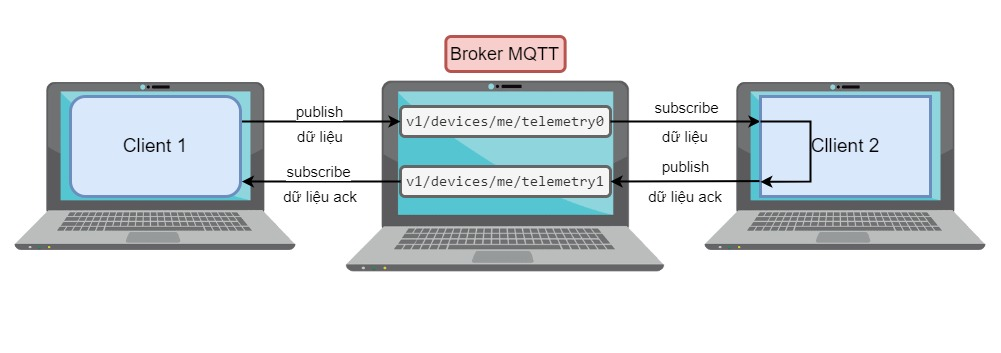
\includegraphics[width=\textwidth]{Images/Comparing_experiment/mqtt_testing_model.jpg}
    \caption{Mô hình hệ thống đo đạc RTT sử dụng MQTT}
    \label{fig:comp_mqtt}
\end{figure}

Từ Client\_1, nhóm sẽ publish dữ liệu với độ dài cho trước tới topic \textbf{v1/devices/me/telemetry0}. Topic này sẽ được lắng nghe (subscribe) bởi Client\_2. Khi Client\_2 nhận được dữ liệu, nó sẽ phản hồi một ack data về \textbf{v1/devices/me/telemtry1}, sau đó được broker gửi ngược về Client\_1. Nhóm sẽ tiến hành lưu thời gian trước khi Client\_1 gửi data (T1) cho tới khi Client\_1 nhận được ack data (T2). RTT sẽ được tính theo công thức sau:

\begin{equation}
    RTT_{MQTT} = T2 - T1
\end{equation}

Để quan sát sự ảnh hưởng của độ dài gói tin lên RTT khi sử dụng giao thức, nhóm lần lượt thử nghiệm gửi từ Client\_1 data có các kích thước là 8b, 32b, 128b, 512b, 2Kb, 8Kb, 32Kb, 128Kb. Với mỗi kích thước data được gửi từ Client\_1, thực nghiệm sẽ được lặp lại 1000 lần để có đánh giá tốt hơn về RTT và các thuộc tính liên quan ứng với mỗi kích thước data. 

Mặt khác, vì MQTT hoạt động theo cơ chế publish - subscribe, khi Client\_1 gửi data tới broker ở dạng publish, Client\_1 sẽ không chờ phản hồi từ Client\_2 gửi xuống mà sẽ gửi ngay data tiếp theo. Chính vì vậy, nhóm có hiện thực cơ chế để đảm bảo chỉ khi Client đã nhận được data ack từ Client\_2 thì mới tiếp tục gửi data ở lần lặp sau để có thể dễ dàng tính toán RTT. Điều này có nghĩa, Client\_1 sẽ thực hiện gửi data và chờ data ack từ Client\_2 suốt 1000 lần với mỗi kích thước data một cách tuần tự, lần lặp tiếp theo chỉ bắt đầu khi Client\_1 đã nhận được data ack từ Client\_2.

Ngoài ra, thực nghiệm sẽ được thực hiện ở 2 trường hợp: điều kiện mạng bình thường và khi mạng có tải cao. Kết nối MQTT giữa broker và client sẽ không có bảo mật, và sử dụng QoS 0.

\subsubsection{OPC-UA}
Để tạo ra sự tương đồng, công bằng về kiến trúc giữa MQTT và OPC-UA trong đo đạc, nhóm đề xuất ra mô hình kiến trúc của OPC-UA như sau:

\begin{figure}[!h]
    \centering
    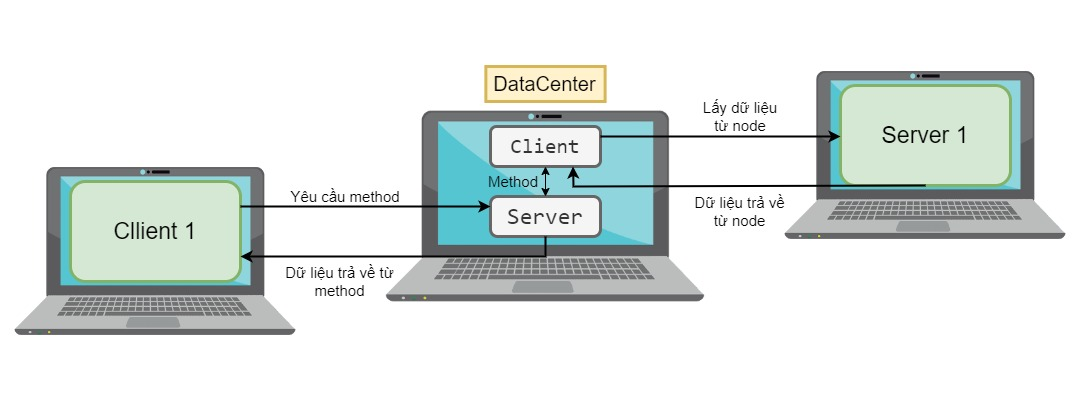
\includegraphics[width=\textwidth]{Images/Comparing_experiment/opcua-architecture.jpg}
    \caption{Mô hình hệ thống đo đạc RTT sử dụng OPC-UA}
    \label{fig:comp_opcua}
\end{figure}

Mô hình kiến trúc có 3 thiết bị chính, bao gồm:
\begin{itemize}
    \item \textbf{Client} : Kết nối tới \textbf{DataCenter} và gọi method để truy xuất về giá trị của node tương ứng
    \item \textbf{DataCenter}: \textbf{DataCenter} là một thiết bị chứa 1 sub client và 1 sub server, với nhiệm vụ tương ứng là kết nói tới \textbf{Server} để lấy ra các node dữ liệu và trả về dữ liệu tương ứng khi method được gọi ở \textbf{Client}
    \item \textbf{Server}: Đây là nơi lưu trữ các node dữ liệu để trả về cho \textbf{DataCenter} khi được truy xuất tới
\end{itemize}

Từ \textbf{Client}, chúng ta kết nối tới sub server của \textbf{DataCenter} và gọi method để lấy về giá trị của node tương ứng ở \textbf{Server} ( Thời điểm này sẽ đánh dấu là T1 ), ở \textbf{DataCenter} sau khi sub sevrer nhận được request call method từ \textbf{Client} thì thực thi một hàm tương ứng với method đã được gọi, hàm này sẽ trả về giá trị mà sub client lấy ra từ node tương ứng ở \textbf{Server} , cuối cùng giá trị node đã được lấy ra sẽ trả về cho \textbf{Client} ( thời điểm sau khi nhận giá trị trả về được đánh dấu là T2). RTT của cả quá trình gửi nhận sẽ được tính theo công thức tương tự như ở MQTT:
\begin{equation}
    RTT_{OPCUA} = T2 - T1
\end{equation}
Tương tự như ở MQTT, để quan sát sự ảnh hưởng của độ dài gói tin lên RTT khi sử dụng giao
thức, nhóm lần lượt thử nghiệm với các node từ \textbf{Server} có các kích thước là
8b, 32b, 128b, 512b, 2Kb, 8Kb, 32Kb, 128Kb. Với mỗi kích thước data, thực nghiệm sẽ được lặp lại 1000 lần để có đánh giá tốt hơn về RTT và các thuộc tính liên quan ứng với mỗi kích thước data. thực nghiệm được thực hiện cũng trong 2 trường hợp: điều kiện mạng ổn định và khi mạng có lượng tải cao. Tốc độ đường truyền sử dụng trong thực nghiệm với OPCUA là tương tự so với khi dùng trong thì nghiệm  MQTT

Tương tự như MQTT, kết nối OPC-UA trong thực nghiệm này sẽ không sử dụng bảo mật, tài khoản hay mật khẩu, là một kết nối vô danh (anonymous).

\subsection{Kết quả thực nghiệm và đánh giá}

Nhóm đã tiến hành thực nghiệm cho hai giao thức trên trên 3 máy tính khác nhau trong cùng một mạng, lưu lại kết quả và sử dụng phần mềm Excel để trích xuất ra các đặc trưng của giá trị RTT cho từng độ dài gói tin và từng trạng thái của mạng. Ở phần kế tiếp, nhóm sẽ trình bày chi tiết kết quả có được sau thực nghiệm và những nhận xét, đánh giá về RTT cho từng giao thức, sau cùng là so sánh chúng với nhau sử dụng biểu đồ trực quan.

\subsubsection{Thực nghiệm MQTT}

Khi thực hiện thực nghiệm với giao thức MQTT trong điều kiện mạng bình thường và điều kiện mạng quá tải, cho kết quả trong bảng sau:

\begin{small}
\begin{longtblr}[
  label = {tblr:ex_mqtt},
  entry = Kết quả thực nghiệm đo RTT của MQTT trong điều kiện mạng bình thường và tải cao,
  caption =  Kết quả thực nghiệm đo RTT của MQTT trong điều kiện mạng bình thường và tải cao,
]{
  width = \linewidth,
  colspec = {Q[117]Q[156]Q[115]Q[90]Q[146]Q[156]Q[152]},
  row{even} = {MintGreen},
  row{3} = {MintGreen},
  row{4} = {Onahau},
  row{5} = {Onahau},
  row{7} = {MintGreen},
  row{8} = {Onahau},
  row{9} = {Onahau},
  row{11} = {MintGreen},
  row{12} = {Onahau},
  row{13} = {Onahau},
  row{15} = {MintGreen},
  row{16} = {Onahau},
  row{17} = {Onahau},
  row{19} = {MintGreen},
  cell{2}{1} = {r=2}{},
  cell{4}{1} = {r=2}{},
  cell{6}{1} = {r=2}{},
  cell{8}{1} = {r=2}{},
  cell{10}{1} = {r=2}{},
  cell{12}{1} = {r=2}{},
  cell{14}{1} = {r=2}{},
  cell{16}{1} = {r=2}{},
  cell{18}{1} = {r=2}{},
  vlines,
  hline{1-2,4,6,8,10,12,14,16,18,20} = {-}{},
}
\textbf{Kích thước} & \textbf{Điều kiện mạng} & \textbf{Trung bình} & \textbf{Trung vị} & \textbf{Độ lệch chuẩn} & \textbf{Giá trị nhỏ nhất} & \textbf{Giá trị lớn nhất} \\
2b                  & Thường                  & 0.1267              & 0.1058            & 0.0652                 & 0.0471                    & 1.1237                    \\
                    & Tải cao                 & 0.3889              & 0.3490            & 0.0602                 & 0.2245                    & 7.3684                    \\
8b                  & Thường                  & 0.1324              & 0.1128            & 0.0657                 & 0.0468                    & 0.7879                    \\
                    & Tải cao                 & 0.3557              & 0.3331            & 0.0073                 & 0.2144                    & 1.0092                    \\
32b                 & Thường                  & 0.1346              & 0.1238            & 0.0569                 & 0.0309                    & 0.6981                    \\
                    & Tải cao                 & 0.3488              & 0.3252            & 0.0074                 & 0.2305                    & 1.0942                    \\
128b                & Thường                  & 0.1374              & 0.1219            & 0.0579                 & 0.0419                    & 0.4157                    \\
                    & Tải cao                 & 0.3887              & 0.3500            & 0.0144                 & 0.2145                    & 1.0979                    \\
                    
512b                & Thường                  & 0.1222              & 0.1057            & 0.0529                 & 0.0469                    & 0.4857                    \\
                    & Tải cao                 & 0.4484              & 0.3985            & 0.0385                 & 0.2174                    & 3.3640                    \\
2Kb                 & Thường                  & 0.1198              & 0.1037            & 0.0473                 & 0.0449                    & 0.4079                    \\
                    & Tải cao                 & 0.4532              & 0.3531            & 0.2768                 & 0.2245                    & 7.1150                    \\
                    % \pagebreak
8Kb                 & Thường                  & 0.1360              & 0.1183            & 0.0620                 & 0.0476                    & 0.5177                    \\
                    & Tải cao                 & 0.4160              & 0.3570            & 0.0439                 & 0.2383                    & 2.8284                    \\
32Kb                & Thường                  & 0.1654              & 0.1456            & 0.0752                 & 0.0529                    & 0.8238                    \\
                    & Tải cao                 & 0.7358              & 0.5465            & 0.2836                 & 0.2813                    & 4.7323                    \\
128Kb               & Thường                  & 0.2393              & 0.2145            & 0.1254                 & 0.1084                    & 1.6087                    \\
                    & Tải cao                 & 2.0553              & 1.8895            & 0.8789                 & 0.6513                    & 9.9854                    
\end{longtblr}
\end{small}

Theo như thực nghiệm, ta thấy có được một số nhận xét sau:

\begin{itemize}
    \item Trong điều kiện bình thường, nhìn chung, khi tăng kích thước gói tin thì RTT trung bình cũng tăng lên. Độ lệch chuẩn với từng kích thước gói tin từ 2 byte tới 32 Kilobytes không chênh lệch quá nhiều, khoảng xấp xỉ 0.0604 giây (60.4ms). Tuy nhiên, khi kích thước gói tin đạt cao hơn - 128Kb, độ lệch chuẩn tăng lên gấp đôi (0.1254s)
    \item Khi tải cao, gói tin có độ dài payload từ 2b tới 128b, RTT trung bình cao gấp xấp xỉ 3 lần so với RTT trung bình ở điều kiện mạng bình thường. Từ 512b tới 8Kb, RTT cao gấp 4 lần. với 32Kb, RTT cao hơn 6 lần và với 128Kb, RTT cao hơn đến 9 lần. Có thể thấy, trong điều kiện tải nặng, khoảng cách về RTT trung bình so với điều kiện bình thường tăng nhanh khi kích thước gói tin tăng.
    \item RTT lớn nhất là 9.9854 giây khi gửi gói tin 128Kb trong điều kiện mạng tải cao. RTT nhỏ nhất là 0.0419 giây khi gửi gói tin 128b trong điều kiện mạng bình thường.
    \item Ngoài ra, trong quá trình thực nghiệm, dù gửi các gói tin lớn với tốc độ cao, MQTT không xảy ra hiện tượng mất gói.

\end{itemize}

Biểu đồ sau đây biểu diễn RTT trung bình khi sử dụng giao thức MQTT gửi các gói tin trong điều kiện mạng bình thường và mạng có tải cao:

%pic here

\begin{figure}[!h]
    \centering
    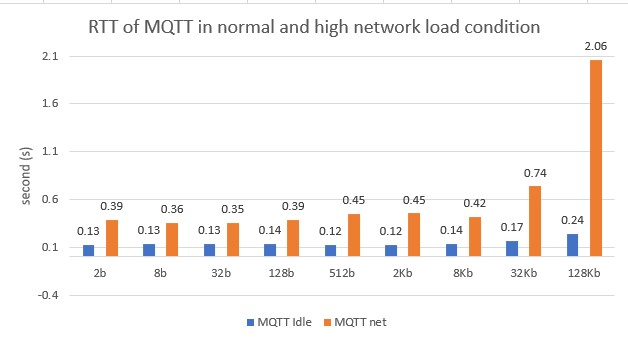
\includegraphics[width=1\textwidth]{Images/Comparing_experiment/mqtt_graph.jpg}
    \caption{Biểu đồ RTT của MQTT trong điều kiện mạng bình thường và quá tải}
    \label{fig:mqtt_graph_0}
\end{figure}

\newpage

\subsubsection{Thực nghiệm OPC-UA}
Khi thực hiện thực nghiệm với giao thức OPCUA trong các điều kiện mạng tương tự như với MQTT, cho kết quả trong bảng sau:

\begin{small}
\begin{longtblr}[
  label = {tblr:ex_opcua},
  entry = Kết quả thực nghiệm đo RTT của OPCUA trong điều kiện mạng bình thường và tải cao,
  caption =  Kết quả thực nghiệm đo RTT của OPCUA trong điều kiện mạng bình thường và tải cao,
]{
  width = \linewidth,
  colspec = {Q[117]Q[156]Q[115]Q[90]Q[146]Q[156]Q[152]},
  row{even} = {MintGreen},
  row{3} = {MintGreen},
  row{4} = {Onahau},
  row{5} = {Onahau},
  row{7} = {MintGreen},
  row{8} = {Onahau},
  row{9} = {Onahau},
  row{11} = {MintGreen},
  row{12} = {Onahau},
  row{13} = {Onahau},
  row{15} = {MintGreen},
  row{16} = {Onahau},
  row{17} = {Onahau},
  row{19} = {MintGreen},
  cell{2}{1} = {r=2}{},
  cell{4}{1} = {r=2}{},
  cell{6}{1} = {r=2}{},
  cell{8}{1} = {r=2}{},
  cell{10}{1} = {r=2}{},
  cell{12}{1} = {r=2}{},
  cell{14}{1} = {r=2}{},
  cell{16}{1} = {r=2}{},
  cell{18}{1} = {r=2}{},
  vlines,
  hline{1-2,4,6,8,10,12,14,16,18,20} = {-}{},
}
\textbf{Kích thước} & \textbf{Điều kiện mạng} & \textbf{Trung bình} & \textbf{Trung vị} & \textbf{Độ lệch chuẩn} & \textbf{Giá trị nhỏ nhất} & \textbf{Giá trị lớn nhất} \\
2b                  & Thường                  & 0.085               & 0.079             & 0.0282                 & 0.0381                    & 0.3556                    \\
                    & Tải cao                 & 0.3148              & 0.2739            & 0.1654                 & 0.1446                    & 3.2371                    \\
                    
8b                  & Thường                  & 0.0848              & 0.0798            & 0.0258                 & 0.0402                    & 0.3536                    \\
                    & Tải cao                 & 0.3167              & 0.2833            & 0.1945                 & 0.0582                    & 3.211                    \\    
                    
32b                 & Thường                  & 0.0832              & 0.0792            & 0.0217                 & 0.0378                    & 0.2048                    \\
                    & Tải cao                 & 0.3363              & 0.3036            & 0.1263                 & 0.1421                    & 1.6016                    \\
                    
128b                & Thường                  & 0.0829              & 0.0790            & 0.0221                 & 0.0461                    & 0.2206                    \\
                    & Tải cao                 & 0.4461              & 0.4061            & 0.1909                 & 0.1843                    & 2.2632                    \\
                    % \pagebreak
                    
512b                & Thường                  & 0.0853              & 0.0796            & 0.0274                 & 0.0434                    & 0.3194                    \\
                    & Tải cao                 & 0.4555              & 0.4224            & 0.1604                 & 0.2081                    & 2.2834                    \\

2Kb                 & Thường                  & 0.0875              & 0.0831            & 0.0271                 & 0.0431                    & 0.4167                    \\
                    & Tải cao                 & 0.3341              & 0.2926            & 0.1501                 & 0.1528                    & 2.7507                    \\
                    
8Kb                 & Thường                  & 0.0884              & 0.0841            & 0.0291                 & 0.0453                    & 0.5967                    \\
                    & Tải cao                 & 0.3185              & 0.2851            & 0.1777                 & 0.1617                    & 4.5577                    \\
            
32Kb                & Thường                  & 0.0959              & 0.0892            & 0.0370                 & 0.0389                    & 0.6254                    \\
                    & Tải cao                 & 0.3370              & 0.3077            & 0.1157                 & 0.1630                    & 1.4815                    \\

128Kb               & Thường                  & 0.1555              & 0.1411            & 0.0586                 & 0.1007                    & 0.6887                    \\
                    & Tải cao                 & 0.8955              & 0.6886            & 0.6410                 & 0.2284                    & 4.0007                    \\
                 
\end{longtblr}
\end{small}

Biểu đồ sau đây biểu diễn RTT trung bình khi sử dụng giao thức OPC-UA gửi các gói tin trong điều kiện mạng bình thường và mạng có tải cao:

\begin{figure}[!h]
    \centering
    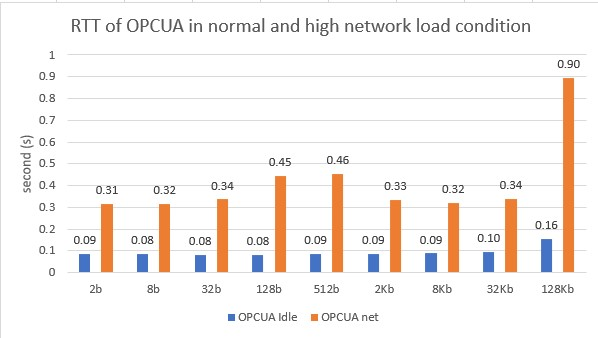
\includegraphics[width=1\textwidth]{Images/Comparing_experiment/rtt-opcua.jpg}
    \caption{Biểu đồ RTT của OPCUA trong điều kiện mạng bình thường và quá tải}
    \label{fig:OPCUA_graph_0}
\end{figure}

Nhìn vào kết quả từ thực nghiệm, ta có một số đánh giá như sau:

\begin{itemize}
    \item Trưởng hợp mạng bình thường, cũng tương tự như MQTT, khi tăng kích thước gói tin thì RTT trung bình cũng tăng lên. Độ lệch chuẩn với từng kích thước gói tin từ 2 byte tới 128 Kilobytes không chênh lệch quá nhiều, khoảng xấp xỉ 0.031 giây (30.1ms). Điều này cho ta thấy được sự ổn định khá cao của OPCUA trong quá trình truyền tải dữ liệu trong điều kiện mạng ổn định.
    
    \item Từ thực nghiệm với MQTT, ta có thể thấy RTT của OPCUA trong các điều kiện thực nghiệm đều thấp hơn so với RTT của MQTT  
    
    \item Trong quá trình thực nghiệm, khi gửi gói tin với tốc độ cao, OPCUA thỉnh thoảng xảy ra hiện tượng mất gói tin, đây là điểm trừ khi so sánh tính toàn vẹn gói tin so với MQTT
\end{itemize}

\subsubsection{So sánh kết quả thực nghiệm}

Sử dụng kết quả từ 2 thực nghiệm với 2 giao thức, nhóm có một số kết quả so sánh sau đây:

\begin{figure}[!h]
    \centering
    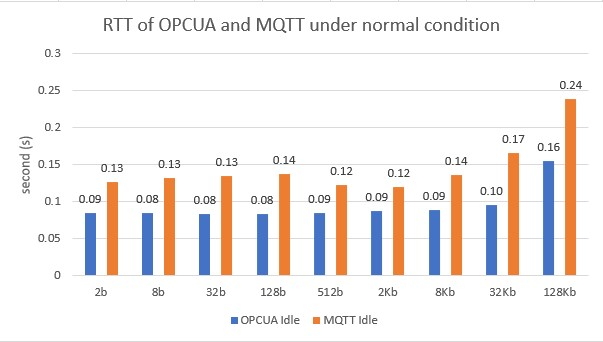
\includegraphics[width=1\textwidth]{Images/Comparing_experiment/comp_opc_mqtt_0.jpg}
    \caption{Biểu đồ RTT trung bình của OPC-UA và MQTT trong điều kiện mạng bình thường}
    \label{fig:comp_opc_mqtt_0}
\end{figure}

\begin{figure}[!h]
    \centering
    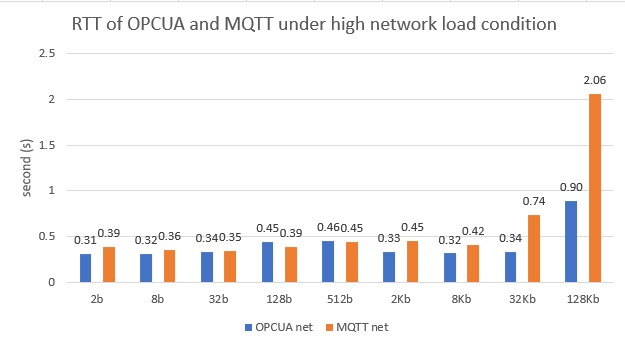
\includegraphics[width=1\textwidth]{Images/Comparing_experiment/comp_opc_mqtt_1.jpg}
    \caption{Biểu đồ RTT trung bình của OPC-UA và MQTT trong điều kiện mạng tải cao}
    \label{fig:comp_opc_mqtt_1}
\end{figure}

% \newpage


Có thể thấy, trong thực nghiệm này, giao thức OPC-UA có RTT tốt hơn MQTT trong hầu hết mọi kích thước gói tin, cả trong điều kiện mạng bình thường và khi mạng có tải cao. Khi kích thước gói tin tăng thì OPC-UA càng thể hiện khả năng gửi nhận nhanh hơn so với MQTT, tuy nhiên, nếu nhanh về tốc độ thì OPC-UA lại bị nhược điểm là đôi lúc xảy ra mất gói khi kích thước dữ liệu lớn trong điều kiện mạng tải cao.

Tiếp đến, biểu đồ boxplot của OPCUA và MQTT được vẽ nên. Ta có một số nhận xét sau:

\newpage

\begin{figure}[!h]
    \centering
    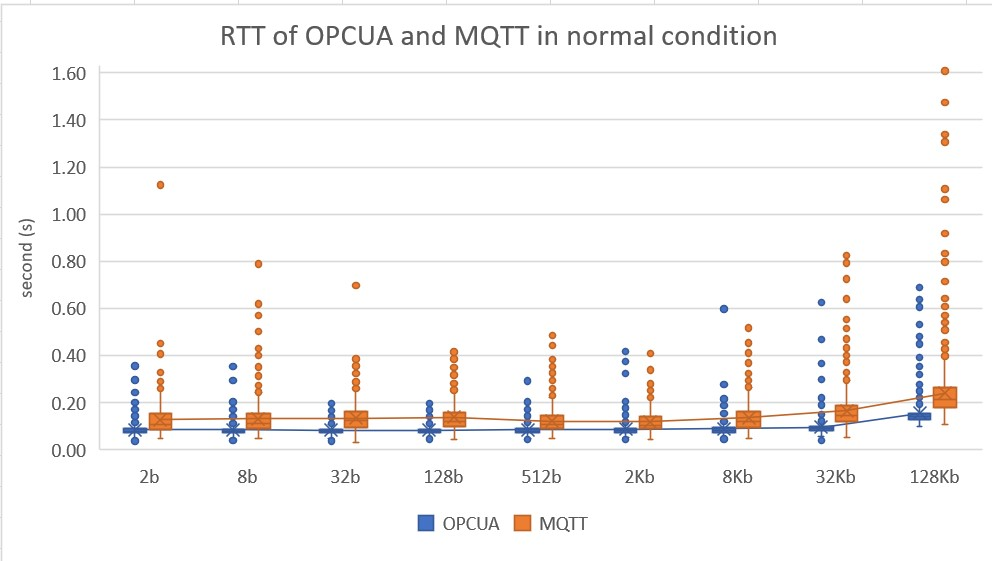
\includegraphics[width=1\textwidth]{Images/Comparing_experiment/comp_opc_mqtt_2.jpg}
    \caption{Biểu đồ Boxplot của OPC-UA và MQTT trong điều kiện mạng bình thường}
    \label{fig:comp_opc_mqtt_2}
\end{figure}

\begin{figure}[!h]
    \centering
    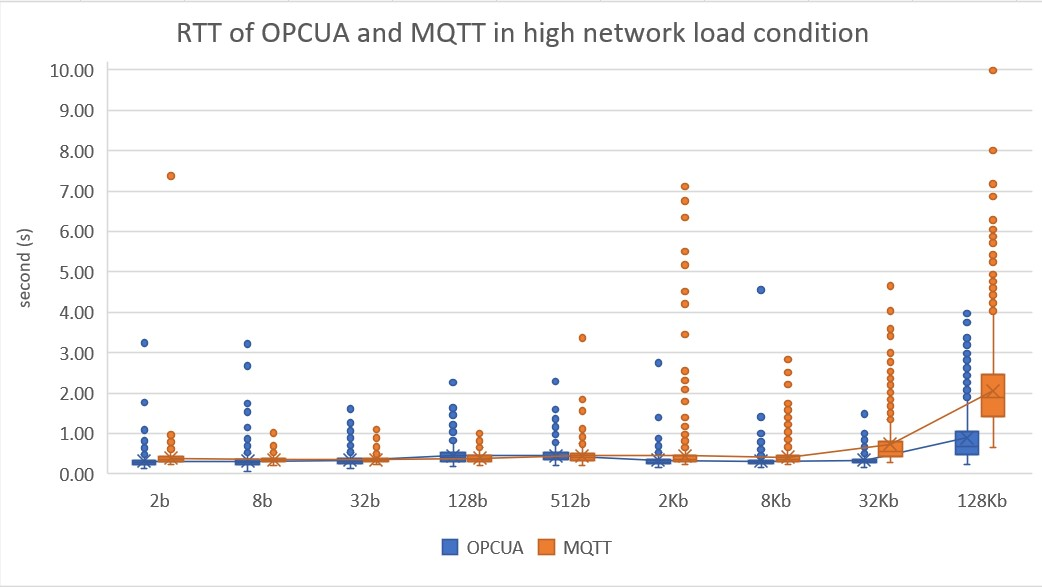
\includegraphics[width=1\textwidth]{Images/Comparing_experiment/comp_opc_mqtt_3.jpg}
    \caption{Biểu đồ Boxplot của OPC-UA và MQTT trong điều kiện mạng tải cao}
    \label{fig:comp_opc_mqtt_3}
\end{figure}

\begin{itemize}
    \item Trong điều kiện mạng bình thường, như nhận xét trước, OPC-UA có RTT trung bình tốt hơn so với MQTT. Điều này dẫn theo các thông số liên quan như Mode, hay trung vị của MQTT cũng lớn hơn so với OPC-UA. Thêm đó, các điểm dữ liệu của OPC-UA tập trung gần trung bình hơn (độ lệch chuẩn nhỏ hơn). Còn với MQTT, các điểm dữ liệu phân tán xa hơn so với giá trị trung bình và cũng có nhiều outliner hơn, cho thấy sự bất ổn định của giao thức khi sử dụng cho các ứng dụng ưu tiên về tốc độ.
    \item Trong điều kiện có tải cao, ở các gói tin có kích thước nhỏ (từ 2b tới 512b), OPC-UA tỏ ra thua kém hơn so với MQTT khi các điểm dữ liệu trở nên phân tán nhiều hơn và nhiều outliner hơn, tuy nhiên giá trị trung bình của RTT vẫn nhỏ hơn so với MQTT. Khi gói tin có kích thước lớn hơn (2Kb trở lên), OPC-UA chiếm lợi thế và các điểm dữ liệu ổn định hơn. Các outlier của OPC-UA không vượt quá 4 giây, do trong hiện thực OPC-UA, timeout cho một request chỉ là 4 giây, quá 4 giây OPC-UA sẽ bỏ gói tin đi. MQTT thoải mái hơn về vấn đề timeout vì chỉ dùng QoS 0, do đó các điểm outlier cũng xa hơn và phân tán hơn, đỉnh điểm ở gói tin 128Kb, RTT lớn nhất của MQTT lên tới 10 giây. MQTT thể hiện khả năng đảm bảo truyền dữ liệu tốt cả khi gói tin lớn và mạng tải cao, nhưng đánh đổi về tốc độ khi thời gian delay khá lớn. OPC-UA có yêu cầu khắt khe về tốc độ và thời gian phản hồi, do đó gửi nhanh hơn MQTT trong các trường hợp khác nhau về độ lớn gói tin, tuy nhiên, do giới hạn của hiện thực OPC-UA trong python, OPC-UA sẽ bỏ gói tin khi request phản hồi lâu hơn 4 giây. 
\end{itemize}


\section{Các nghiên cứu liên quan}

Sự phát triển mạnh mẽ của ngành công nghiệp 4.0, đặc biệt là AI, IoT và gần đây IIoT (Industrial Internet of things) đang được thúc đẩy với các cải tiến, sáng kiến mới. OPCUA từ lâu đã là một giao thức phổ biến dùng trong môi trường công nghiệp, cũng đang không ngừng cải thiện với tham vọng trở thành một giao thức truyền thông mạnh mẽ trong IIoT, đem lại khả năng tích hợp cao với mọi thiết bị, trong mọi môi trường khác nhau, tạo thành một hệ sinh thái OPC UA phủ khắp từ các thiết bị trong nhà máy tới giao tiếp trên đám mây. Việc tích hợp OPC UA rộng rãi sẽ nhằm giảm bớt sự phức tạp và phiền toái khi thiếu đi sự đồng nhất trong giao tiếp giữa các thiết bị với vô số các chuẩn giao tiếp công nghiệp trước đó. Tận dụng những đặc điểm nổi trội của OPC UA, nhiều nghiên cứu đã được đề ra kết hợp với IoT, IIoT, AI và Digital twin. Ahmad Abdelstattar \cite{abdelsattaropcgateway} đề xuất một kiến trúc dạng client-gateway để tăng tính mở rộng của kiến trúc OPC UA dạng client-server mặc định, bằng cách tạo thêm một gateway trung gian chạy OPC UA client. Gateway trung gian này sẽ thu thập dữ liệu từ các OPC UA server chạy trên thiết bị nhúng hoặc trên các điều khiển công nghiệp (industrial controller), từ đó làm nơi tập trung dữ liệu trung chuyển đi cho các ứng dụng trên điện toán đám mây đối với người dùng ở xa, hoặc cho ứng dụng Digital twin cho người dùng cục bộ thông qua CAD model, SCADA (Supervisory Control and Data Acquisition), cho phép họ điều khiển thiết bị thời gian thực và chính xác. Trong bài báo của mình, tác giả cũng đã hiện thực một ví dụ điều khiển FESTO MPS (Modular Production System) với một OPC server chạy trên PLC siemens S7-1516. Một máy tính (PC) trở thành gateway chạy OPC client nhằm thu thập dữ liệu từ thiết bị, trên đó chạy một HMI/SCADA để giúp người dùng theo dõi dữ liệu. Bài báo cũng chỉ ra rằng việc tập trung dữ liệu và xử lý ở gateway hiệu năng cao sẽ giảm bớt độ phức tạp ở các thiết bị điều khiển, từ đó cung cấp dữ liệu thời gian thực tốt hơn. Phần hiện thực của bài báo còn hạn chế do giới hạn về tốc độ gửi dữ liệu của OPC server trên PLC, rắc rối về đồng bộ thời gian và thiếu mô hình 3D để tượng trưng cho Digital Twin nhằm theo dõi hoạt động thiết bị.

Mặt khác, Amirashkan Haghshenas \cite{haghshenaspredictivewindstore} xây dựng một hệ thống Digital Twin của trang trại cối xoay gió ngoài biển sử dụng OPC UA làm giao thức truyền nhận. Tác giả bài báo cho rằng OPC UA thỏa mãn được các yêu cầu phi chức năng mà hệ thống đề ra: cung cấp khả năng truyền dữ liệu bảo mật, đáng tin cậy và hỗ trợ thu thập dữ liệu thời gian thực. Kiến trúc hệ thống bao gồm một Node-RED thu thập các dữ liệu cảm biến gắn liền với bo mạch nhúng Arduino, đồng thời chạy một OPC UA client. Từ NodeRed có thể cung cấp dữ liệu cần thiết cho giao diện điều khiển 2D, và sử dụng OPC UA, truyền dữ liệu trực tiếp lên một OPC UA server. OPC UA server lại đóng vai trò như một trung tâm dữ liệu, đưa dữ liệu lên hai ứng dụng, một ứng dụng 3D cho mô phỏng và và ứng dụng 3D thực tế ảo tăng cường (Augmented Reality). Hai ứng dụng 3D đều được xây dựng sử dụng Unity Engine và chạy OPC client để kết nối tới Node-Red. Bài báo tập trung nhiều vào việc xây dựng ứng dụng Digital Twin với nhiều chức năng như mô phỏng vật lý theo điều khiển của người dùng, chạy mô phỏng phức tạp dựa trên dữ liệu mô phỏng từ Matlab Simulink, dự đoán dựa trên tập dữ liệu lịch sử và điều khiển thiết bị trực tiếp thông qua OPC UA. Ứng dụng thể hiện được khả năng mạnh mẽ, không chỉ thể hiện trạng thái thiết bị, còn có thể dựa vào dữ liệu thu thập để đưa ra dự đoán lỗi nhiệt độ hoặc lỗi rung động bằng một số giải thuật.

Ở đồ án trước, nhóm cũng đã xây dựng một kiến trúc điều khiển cánh tay robot đơn giản gồm ba khối: control để điều khiển thiết bị, datacenter để tổng hợp dữ liệu và một ứng dụng điện thoại 2D để gửi lệnh điều khiển xuống datacenter nhằm thay đổi trạng thái cánh tay robot. nhóm đã thành công trong việc sử dụng giao thức OPC UA để điều khiển thiết bị bằng ứng dụng điện thoại, tuy nhiên kết quả đó cũng có nhiều mặt hạn chế. Thứ nhất là phần thiết bị - cánh tay robot thiếu đi sự phản hồi về trạng thái thật của cánh tay, do đó nhóm không thể biết chính xác trạng thái của cánh tay đang ở vị trí nào và góc xoay bao nhiêu. Thứ hai, cấu trúc dữ liệu điều khiển cánh tay trên OPC UA server được thực hiện sơ sài và đơn giản, do đó tạo ra nhiều khó khăn trong việc đồng bộ dữ liệu giữa ba khối. Thứ ba, Datacenter được viết phụ thuộc nhiều vào node ID của cấu trúc dữ liệu trên khối control, do đó nếu khối control thay đổi về số lượng node hay cách sắp xếp sẽ ảnh hưởng ngược lại tới khối Datacenter. Thứ tư là ứng dụng điện thoại chỉ ở mức ứng dụng 2D, ngoài ra khi điều khiển cũng không có cách nào biết liệu điều khiển có thành công hay không do thiếu sự phản hồi từ thiết bị. 

Trong luận văn này, đồ án của nhóm tiếp tục sử dụng lại kiến trúc có sự xuất hiện của Datacenter - một khối trung gian làm trung tâm lưu trữ, truyền và đồng bộ dữ liệu. Với việc sử dụng Datacenter, nhóm có thể kết nối điều khiển nhiều thiết bị hơn, các thiết bị có thể được điều khiển bởi mạch lập trình nhúng hoặc PLC chạy OPC server. Trên Datacenter, sẽ có nhiều client OPC UA nhỏ để kết nối với các OPC server, và đồng thời cung cấp một server OPC UA duy nhất để các ứng dụng cần thu thập dữ liệu truy cập tới. Datacenter cũng được lập trình để không bị ảnh hưởng bởi sự thay đổi của module Control. Hơn nữa, nhóm có cơ hội cải tiến hệ thống gồm một thiết bị là cánh tay robot JetMax mạnh mẽ chạy OPC server, kết nối với một Datacenter, và một ứng dụng thực tế ảo (Virtual Reality) chạy OPC client kết nối với Datacenter. Cánh tay robot được nhóm tích hợp một số ứng dụng AI đơn giản như gắp rác bán tự động, theo dõi khối màu, xếp chồng khối gỗ và quan trọng là khả năng tự phản hồi trạng thái dưới sự điều khiển của ROS. Các chức năng này được cung cấp và sử dụng được thông qua OPC Server trên cánh tay robot và trên ứng dụng thực tế ảo VR. Thêm vào đó, Ứng dụng VR được xây dựng trên Unity Engine, đem lại cảm giác điều khiển chân thực hơn cho người dùng và liên tục cập nhật theo trạng thái thật của thiết bị thực tế. Việc sử dụng giao thức OPC UA trong môi trường mạng cục bộ giúp truyền nhận dữ liệu nhanh hơn, giúp nhóm xây dựng nên ứng dụng điều khiển thời gian thực hiệu quả. 

